\chapter{Esperimenti Classificazione}\label{ch:chapter2}
\section{Dataset}
\subsection{Descrizione del dataset }
Il Dataset su cui sono stati effettuati gli esperimenti descritti in questo elaborato di tesi è il medesimo usato da \citet{soccerNet}.
Tale Dataset è formato da \textbf{500 partite}, per un totale di \textbf{764 ore} di gioco, prese dai principali campionati europei durante le tre stagioni 2014-2015, 2015-2016 e 2016-2017.
\\Maggiori dettagli sui campionati e sulla suddivisone delle partite sono foriniti nella tabella \textbf{\ref{table: Dataset}}
\\Per assicurare un corretto confronto con la baseline, ho utilizzato la medesima suddivione utilizzata nel loro paper \cite{soccerNet} nella quale: le partite del dataset sono state divise randomicamente in \textbf{300}, \textbf{100}, \textbf{100} per \textbf{training}, \textbf{validation} e \textbf{testing}, assicurandosi in questo modo una distribuzione similare degli eventi in ogni porzione di dataset.
\begin{table}[H]
\caption{Suddivisone delle partite per lega e anno nel nostro Dataset}
\centering
\begin{tabular}{c| | c|c|c | | c}
\multicolumn{1}{c}{}&\multicolumn{3}{c}{Stagioni}& \\
Lega & 14/15 & 15/16 & 16/17 & \textbf{Total} \\
\hline
EN - EPL & 6 & 49 & 40 & \textbf{95} \\
ES - LaLiga & 18 & 36 & 63 & \textbf{117} \\
FR - Ligue 1 & 1 &  3 & 34 & \textbf{38} \\
DE - BundesLiga & 8 & 18 & 27 & \textbf{53} \\
IT - Seria A & 11 & 9 & 76 & \textbf{96} \\
EU - Champions & 37 & 45 & 19 & \textbf{101} \\
\hline
Total & \textbf{81} & \textbf{160} & \textbf{259} & \textbf{500} \\ [1ex]

\end{tabular}
\label{table: Dataset}
\end{table}
Dai video delle partite sono state poi estratte le features mediante la rete neurale ResNET con il procedimento descritto in precedenza.
\subsection{Label}
Oltre ai video, il Dataset è formato dalle \textbf{annotazioni} (\textbf{label}), le quali sono state inizialmente ottenute effetuando il \textit{parsing} dei report delle partite direttamente sui siti delle varie leghe calcistiche.
\\Tuttavia la precisione delle annotazioni così ottenute non è abbastanza elevata per i nostri propositi essendo di un \textbf{minuto}, a causa di ciò si sono dovuti riannotare \textbf{manualmente} gli eventi, all'interno del minuto già noto, per ottenere una precisione di un \textbf{secondo}.
\\Per essere in grado di fare ciò, si sono dovuti definire gli esatti istanti temporali che corrispondono alle azioni di nostro interesse.
\\Definiamo quindi:
\begin{itemize}
\item L'evento \textbf{Goal} come l'istante in cui la palla oltrepassa la linea di porta
\item L'evento \textbf{Cartellino} come l'instante in cui l'arbitro estrae il cartellino giallo
\item L'evento \textbf{sostituzione} l'istante come in cui il giocatore entra nel terreno di gioco
\end{itemize}
L'unica eccezione alle definizioni sovracitate sono le sostituzioni avvenute durante l'\textbf{intervallo}, per le quali è impossibile dare una definzione che corrisponda con quanto accade in video.
\subsection{Suddivisone minuto per minuto}
Il nostro dataset formato, come detto sopra, da 500 partite e 764 ore di video, per poter essere elaborato da un rete neurale è stato poi suddiviso in porzioni disgiunte aventi la \textbf{durata di un minuto}.
\\In questa fase il nostro è un problema di \textbf{classificazione}, in cui un singolo campione è formato da \textbf{120 raggruppamenti} di features ed è annotato con gli eventi occorrenti in quel minuto.
\\Ovviamente essendo molto più probabile che in un minuto di una partita non accada niente piuttosto che sia presente un'azione da noi ricercata, il nostro dataset è decisamente sbilanciato, esso infatti nel training set contiene:
\begin{itemize}
\item \textbf{1246} campioni in cui è presete un \textbf{cartellino}
\item \textbf{1558} campioni in cui è prsente una \textbf{sostituzione}
\item \textbf{960} campioni in cui è presente un \textbf{goal}
\item \textbf{23750} campioni di \textbf{background}, ovvero in cui non avviene nessuna delle tre azioni sopracitate
\end{itemize}
È importante notare inoltre come ben \textbf{115} campioni abbiano label multiple, per una corretta classificazione è necessario che il modello ammetta la possbilità di classificare questi campioni nel modo corretto.
\section{Metriche}
\subsection{Mean Average Precision}
La metrica usata nel paper di riferimento con cui ci andremo a confrontare è la metrica denominata \textbf{Mean Average Precision} (\textbf{mAP}). Per il calcolo di tale metrica viene utilizzata la \textbf{precision-recall curve}.
\\Prima di procere oltre è bene introdurre i concetti di \textbf{precision} e \textbf{recall}:
\begin{itemize}
\item La metrica \textbf{precison} misura quanto accurate sono le tue predizioni, ovvero la precentuale di previsioni corrette.
\begin{equation}
Precision=\frac{True Positives}{True Positives + False Positives}
\label{Precision}
\end{equation}
\item La metrica \textbf{recall} misura quanto correttamente riesci a trovare tutti i positivi, può essere pensata quindi come l'abilità di un modello di trovare i punti di interesse di un dataset.
\begin{equation}
Recall=\frac{True Positives}{True Positives + False Negatives}
\label{Recall}
\end{equation}
\end{itemize}
La metrica \textbf{Average-Precision} (\textbf{AP}) è defnitita come l'area al di sotto della curva precision-recall.
\\Infine la metrica \textbf{Mean Average Precision} è definita come la \textbf{media} tra i valori delle \textbf{AP} per ogni evento. 
\\Nel nostro caso quindi sono state calcolate \textbf{tre} AP (per \textbf{goal}, \textbf{sostituzioni} e \textbf{cartellini}) e successivamente è stata fatta la media aritmetica.
\\Questa metrica sfortunatamente non mi è stato possibile utilizzarla in fase di training (e quindi validazione), questo a causa del fatto che la mAP non è nativamente supportata in Keras, per poterla utilizzare è stato quindi necessario importare tale metrica da \textbf{Tensorflow}.
\\Le metriche di Tensorflow \textbf{non supportano} tuttavia i dati costruiti mediante \textbf{funzioni generatrici}, fatto invece necessario a causa della pesantezza dei nostri dati.
\\Per questo motivo per effettuare il \textit{fine-tuning} della mia rete neurale è stato necessario utilizzare una metrica diversa.
\subsection{F1}
La metrica utilizzata in fase di validazione è stata quindi la \textbf{F1}, essa combina le metriche di \textbf{Precision} e \textbf{Recall} sopra definite ed ha la seguente espressione:
\begin{equation}
F1=2*\frac{Precision * Recall}{Precision + Recall}
\label{F1}
\end{equation}
Nel nostro caso, dato che a noi interessa principlamente indivduare le porzioni di partita in cui accade un evento saliente, tale metrica è stata calcolata solamente sulle \textbf{tre} label di nostro interesse \textbf{trascurando} quella di background.
\\La metrica \textbf{F1} è stata inoltre utilizzata nel capitolo \ref{ch:chapter3} nel task di \textbf{localizzazione}
\section{Baseline}
I \textbf{risultati} ottenuti dalla baseline mediante le varie tecniche di pooling precedentemente accennate ed utilizzando le features estratte con ResNET sono elencati di seguito.\cite{soccerNet} 
\\Inizialmente sono stati effettuati degli esperimenti con i metodi di pooling senza effettuare alcun tipo di fine-tuning, in particolare sui metodi proposti da \citet{MiechPooling} (\textbf{SoftDBOW}, \textbf{NetFV}, \textbf{NetVLAD} e \textbf{NetRVLAD}) sono stati usati \textbf{k=16} cluster.
\\I risultati sono riassunti nella tabella \textbf{\ref{table: baselinek16}}.
\begin{table}[ht]
\caption{Risultati per i diversi metodi di pooling}
\centering
\begin{tabular}{c| | c}
\textbf{Pooling} & \textbf{mAP} \\
\hline
\textbf{Mean Pool.} & 40.2 \\
\textbf{Max Pool.} &  52.4\\
\textbf{CNN} & 53.5\\
\textbf{SoftDBOW} & 48.9\\
\textbf{NetFV} & 64.4\\
\textbf{NetRVLAD} & \textbf{65.9}\\
\textbf{NetVLAD} & 65.2\\ [1ex]

\end{tabular}
\label{table: baselinek16}
\end{table}
\\Ovviamente all'aumentare dei cluster aumenta la potenza espressiva del sistema, generando con buona prababilità un aumento di prestazioni.
\begin{table}[ht]

\caption{mAP al variare del numero di cluster k per i metodi di pooling proposti da \citet{MiechPooling}}
\label{table: baselinek16to512}
\centering
\begin{tabular}{c| | c|c|c |  c}
&\multicolumn{4}{c}{\textbf{Metodi di Pooling}} \\
k & \textbf{SoftBOW} & \textbf{NetFV} & \textbf{NetRVLAD} & \textbf{NetVLAD} \\
\hline
\textbf{16}& 54.9 & 63.0 & 64.4 & 65.2 \\
\textbf{32} & 57.7 & 64.0 & 63.8 & 65.1 \\
\textbf{64}& 58.8 &  64.1 & 65.3 & 65.2 \\
\textbf{128}& 60.6 & 64.4 & 67.0 & 65.6 \\
\textbf{256}& 61.3 & 63.8 & 67.7 & 67.0 \\
\textbf{512} & 62.0 & 62.1 & 67.4 & \textbf{67.8} \\[1ex]

\end{tabular}
\end{table}
\\Nella tabella \textbf{\ref{table: baselinek16to512}} infatti si vede come, inizialmente, all'aumentare delle dimensioni dei cluster migliorino le prestazioni, tuttavia oltre i 256 cluster esse iniziano a stabilizzarsi a causa dell'\textbf{overfitting}.
\\Inoltre la \textbf{complessità computazionale} cresce \textbf{linearmente} col numero dei cluster.\\
\linebreak
Il miglior risultato della baseline, quello quindi con cui ci siamo andati a confrontare, è ottenuto mediante \textbf{NetVLAD} con \textbf{k=512} cluster.
\\Come evidenziato nella tabella \textbf{\ref{table: baselinek16to512}} tale modello sul nostro dataset ha una mAP del \textbf{67.8\%}.
\section{I miei risultati}
Il modello che è stato utlizzato per cercare di migliorare i risultati ottenuti con la baseline, è stato precedentemente descritto nei dettagli.
\\Si tratta di una rete neurale ricorrente formata da tre layer GRU bidirezionali con l'aggiunta del layer di ouput.
\subsection{Training and Validation}
Come detto in precedenza a causa dell'incompatibilità tra le metriche di Tensorflow e i dati costruiti mediante generatori in Keras non mi è stato possibile  utilizzare la metrica mAP in fase di training del mio modello.
\\Per questo motivo nel grafico in figura \textbf{\ref{figure : trainingvalf1}} viene rappresentato l'andamento della metrica \textbf{f1} (denominata \textbf{f1m} per sottolinare il fatto che non viene considerata la label di background).
\\Nella figura \ref{figure : trainingvalloss} possiamo vedere come la loss function inizi a crescere dopo circa \textbf{10} epoche, facendoci pensare che il modello da li in poi inizi a peggiorare a causa dell'overfitting.
\\Tuttavia nella figura \textbf{\ref{figure : trainingvalf1}} possiamo vedere come la metrica f1 continui a migliorare anche dopo 10 epoche, stabilizzandosi circa alla trentsima epoca e avendo il miglior risultato all'epoca numero \textbf{34}.
\\Questa discrepanza è dovuta alla \textbf{polarizzazione}, verso 0 o verso 1, delle probabilità di output del mio modello.
\begin{figure}[ht]
\centering
\caption{Training and validation loss}
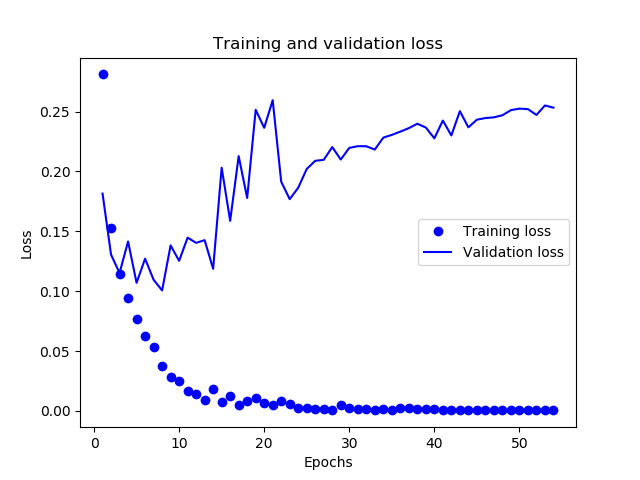
\includegraphics[width=\linewidth]{img/training-validation-loss.png}
\label{figure : trainingvalloss}
\end{figure}
\begin{figure}[H]
\centering
\caption{Training and validation f1m}
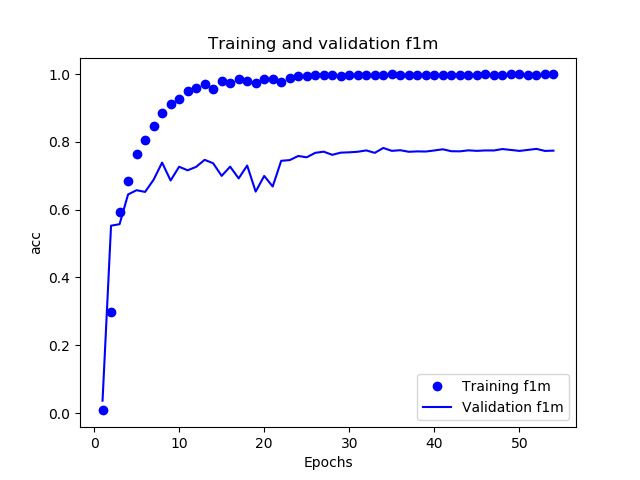
\includegraphics[width=\linewidth]{img/training-validation-f1m.png}
\label{figure : trainingvalf1}
\end{figure}
\subsection{Test}
Per verificare definitivamente la bontà del nostro modello è stato necessario testarlo sulla porzione di dataset riservata a tali propositi. 
\\In questa fase la metrica di riferimento torna a essere la \textbf{mAP}.
\begin{table}[ht]
\label{table: test}
\caption{Risultati sul test set}
\centering
\begin{tabular}{c|c|c||c}
\multicolumn{3}{c}{\textbf{AP}}\\
\textbf{Cartellino} & \textbf{Sostituzione} & \textbf{Goal} & \textbf{mAP} \\
\hline
77.6& 78.7 & 82.8 & \textbf{79.7} \\ [1ex]
\end{tabular}
\end{table}
\\Considerando che il risultato migliore della baseline contro cui mi sono confrontato è del \textbf{67.8\%}, il 
risultato ottenuto possiamo ritenerlo soddisfacente, essendo infatti un miglioramento di oltre il \textbf{10\%}.